\documentclass[11pt,a4paper,oneside]{report}             % Single-side
%\documentclass[11pt,a4paper,twoside,openright]{report}  % Duplex

\usepackage{enumerate}
\usepackage{listings}
\usepackage{color}
\usepackage{graphics}
\usepackage{epsfig}
\usepackage{amsmath}
\usepackage{amssymb}
\usepackage[thmmarks]{ntheorem}
\usepackage[utf8]{inputenc}
\usepackage[T1]{fontenc}
\usepackage[english]{babel}
\usepackage{lastpage}
\usepackage{anysize}
\usepackage{sectsty}
\usepackage{setspace}
\usepackage[hang]{caption}
\usepackage{hyperref}

%--------------------------------------------------------------------------------------
% Main variables
%--------------------------------------------------------------------------------------
\newcommand{\vikszerzo}{Viktória Nemkin}
\newcommand{\vikkonzulens}{dr.~Márk Asztalos, András Kárpinszky}
\newcommand{\vikcim}{Implementation of the optimization of multi-variable target functions through an example timetabling application}
\newcommand{\viktanszek}{Department of Automation and Applied Informatics}
\newcommand{\vikdoktipus}{BSc. Thesis}


\pagestyle{plain}
\setlength{\parindent}{0pt}
\setlength{\parskip}{8pt plus 3pt minus 3pt}

\marginsize{35mm}{25mm}{15mm}{15mm}
\setcounter{secnumdepth}{0}
\sectionfont{\large\upshape\bfseries}
\setcounter{secnumdepth}{2}
\singlespacing
\frenchspacing

\hypersetup{
    bookmarks=true,
    unicode=false,
    pdftitle={\vikcim},
    pdfauthor={\vikszerzo},
    pdfsubject={\vikdoktipus},
    pdfcreator={\vikszerzo},
    pdfproducer={Producer},
    pdfkeywords={keywords},
    pdfnewwindow=true,
    colorlinks=true,
    linkcolor=black,
    citecolor=black,
    filecolor=black,
    urlcolor=black
}

\lstset{
	basicstyle=\scriptsize\ttfamily,
	keywordstyle=\color{black}\bfseries\underbar,
	identifierstyle=,
	commentstyle=\color{white},
	stringstyle=\scriptsize\sffamily,
	showstringspaces=false,
	aboveskip=3pt,
	belowskip=3pt,
	columns=fixed,
	backgroundcolor=\color{lightgray},
}

\def\lstlistingname{lista}	

\newcommand{\code}[1]{{\upshape\ttfamily\scriptsize\indent #1}}

\newcommand{\figref}[1]{\ref{fig:#1}.}
\renewcommand{\eqref}[1]{(\ref{eq:#1})}
\newcommand{\listref}[1]{\ref{listing:#1}.}
\newcommand{\sectref}[1]{\ref{sect:#1}}
\newcommand{\tabref}[1]{\ref{tab:#1}.}

\DeclareMathOperator*{\argmax}{arg\,max}
\DeclareMathOperator{\sign}{sgn}
\DeclareMathOperator{\rot}{rot}
\definecolor{lightgray}{rgb}{0.95,0.95,0.95}

\author{\vikszerzo}
\title{\viktitle}

\captionsetup[figure]{
width=.75\textwidth,
aboveskip=10pt}

\renewcommand{\captionlabelfont}{\small\bf}
\renewcommand{\captionfont}{\footnotesize\it}

\begin{document}
\singlespacing

\pagenumbering{arabic}
\onehalfspacing
%--------------------------------------------------------------------------------------
%	The title page
%--------------------------------------------------------------------------------------
\begin{titlepage}
\begin{center}

\includegraphics[width=60mm,keepaspectratio]{figures/BMElogo.png}\\
\vspace{0.3cm}
\textbf{Budapesti M�szaki �s Gazdas�gtudom�nyi Egyetem}\\
\textmd{Villamosm�rn�ki �s Informatikai Kar}\\
\textmd{\viktanszek}\\[5cm]

\vspace{0.4cm}
{\huge \bfseries \vikcim}\\[0.8cm]
\vspace{0.5cm}
\textsc{\Large \vikdoktipus}\\[4cm]

\begin{tabular}{cc}
 \makebox[7cm]{\emph{K�sz�tette}} & \makebox[7cm]{\emph{Konzulens}} \\
 \makebox[7cm]{\vikszerzo} & \makebox[7cm]{\vikkonzulens}
\end{tabular}

\vfill
{\large \today}
\end{center}
\end{titlepage}



\tableofcontents
\newpage
%--------------------------------------------------------------------------------------
% Nyilatkozat
%--------------------------------------------------------------------------------------
\begin{center}
\large
\textbf{HALLGAT�I NYILATKOZAT}\\
\end{center}

Alul�rott \emph{\vikszerzo}, szigorl� hallgat� kijelentem, hogy ezt a szakdolgozatot/ diplomatervet \textcolor{blue}{(nem k�v�nt t�rlend�)} meg nem engedett seg�ts�g n�lk�l, saj�t magam k�sz�tettem, csak a megadott forr�sokat (szakirodalom, eszk�z�k stb.) haszn�ltam fel. Minden olyan r�szt, melyet sz� szerint, vagy azonos �rtelemben, de �tfogalmazva m�s forr�sb�l �tvettem, egy�rtelm�en, a forr�s megad�s�val megjel�ltem.

Hozz�j�rulok, hogy a jelen munk�m alapadatait (szerz�(k), c�m, angol �s magyar nyelv� tartalmi kivonat, k�sz�t�s �ve, konzulens(ek) neve) a BME VIK nyilv�nosan hozz�f�rhet� elektronikus form�ban, a munka teljes sz�veg�t pedig az egyetem bels� h�l�zat�n kereszt�l (vagy autentik�lt felhaszn�l�k sz�m�ra) k�zz�tegye. Kijelentem, hogy a beny�jtott munka �s annak elektronikus verzi�ja megegyezik. D�k�ni enged�llyel titkos�tott diplomatervek eset�n a dolgozat sz�vege csak 3 �v eltelte ut�n v�lik hozz�f�rhet�v�.

\begin{flushleft}
\vspace*{1cm}
Budapest, \today
\end{flushleft}

\begin{flushright}
 \vspace*{1cm}
 \makebox[7cm]{\rule{6cm}{.4pt}}\\
 \makebox[7cm]{\emph{\vikszerzo}}\\
 \makebox[7cm]{hallgat�}
\end{flushright}
\thispagestyle{empty}

\vfill
\clearpage
\thispagestyle{empty} % an empty page


\chapter*{Kivonat}\addcontentsline{toc}{chapter}{Kivonat}

\vfill

\chapter*{Abstract}\addcontentsline{toc}{chapter}{Abstract}

\vfill


%----------------------------------------------------------------------------
\chapter*{Bevezet�}\addcontentsline{toc}{chapter}{Bevezet�}
%----------------------------------------------------------------------------

A bevezet� tartalmazza a diplomaterv-ki�r�s elemz�s�t, t�rt�nelmi el�zm�nyeit, a feladat indokolts�g�t (a motiv�ci� le�r�s�t), az eddigi megold�sokat, �s ennek t�kr�ben a hallgat� megold�s�nak �sszefoglal�s�t.

A bevezet� szok�s szerint a diplomaterv fel�p�t�s�vel z�r�dik, azaz annak r�vid le�r�s�val, hogy melyik fejezet mivel foglalkozik.


\chapter{Requirement specification}

I have met with Erzsébet Győri, the timetable creator of our faculty and we discussed how she currently creates the timetables and what specific requirements and requests arise during the process and what my system shall be capable of.

Below is a summary of these.

\begin{itemize}

\item The user shall be able to record the buildings and rooms in the system.
\item The user shall be able to record the departments, their faculty members and which classes and course types they can teach.
\item The user shall be able to record the years of the students.
\item The user shall be able to record the classes for every year and the courses from the given classes.
\item Every practice session shall be able to be scheduled independently.
\item For every timeslot, the maximum amount of classes shall not have more capacity than the entire year of students.
\item During breaks students shall be able to comfortably walk from the current room to the next in the available time. Commutes from building K to building I and back shall be reduced or eliminated.
\item For practice sessions of a given class, all of them shall be either before or preferably after the seminar for the given week.  
\item Some practice sessions have an assigned teacher, and some don't (for student demonstrators). When the teacher is assigned the class shall not conflict with another class of the same teacher.
\item Some faculties have a low number of student demonstrators so they can't handle a large number of parallel practice sessions.  
\item Every department and faculty member shall be able to specify when they are available to teach and be given a schedule accordingly.
\item For all courses, the departments shall be able to specify when they can be scheduled.
\item Every faculty member shall be able to specify the locations (buildings) they would prefer to teach in.
\item Some classes have multiple seminars and designated practice sessions depending on the chosen seminar. These practice sessions shall be scheduled depending on their corresponding seminars.
\item We have rooms with capacities, described as XL (400 students), L (200 students), M (100 students), S (35 students), and XS (20 students) and special laboratory rooms. Each course shall have a suitable sized room assigned to it.
\begin{itemize}
    \item XL rooms are suitable for holding large seminars for the first few years of students.
    \item L rooms are fitting for specialisation seminars for students in a higher year.
    \item M rooms are good for smaller seminars, consultations or electives.
    \item S rooms are for practice sessions.
    \item XS rooms are suitable for a smaller number of students, like IMSC groups.
    \item Laboratory rooms are either owned and assigned by the departments or made available by the HSZK (in building R).
\end{itemize}
\item Some rooms are only available for a given period (Q-I, for example - is shared with GTK). The software shall be able to take room availabilities into account.
\item The software shall be able to integrate with the Neptun system. It shall be able to download the list of courses for a given semester, schedule them and output the result in a suitable format for Neptun.
\item Laboratory courses have a preferred order during the week. This is so they don't have to switch back and forth between the equipment.  
\item Teacher's schedules shall not have more than a specified number of hours of class for any given day.
\item Exam periods shall be scheduled as well.  
\item For the first year students are arranged in groups. Each student group has an assigned timetable so they take their practice sessions and laboratory classes together.
\item The schedule shall not have hole-hours for first-year students.
\item Student groups have a lunch break from 12 pm to 1 pm.
\item IMSC student groups shall be taken into account. They are separated and they, have their own timetable.
\item There shall be separate software for the data entry (client) and the solver (server).
\item The client shall be able to run on low resources on older Windows versions as well as Windows 10.
\item The server shall run on Linux and make use of multiple available processors.
\item The generated schedules shall have no conflicts for the years of students, the faculty members and the rooms.
\end{itemize}

The requirements above are complex and expansive. For the current semester I decided to focus on the following subset of these:

\begin{itemize}
\item The user shall be able to record the buildings and rooms in the system.
\item The user shall be able to record the departments, their faculty members and which classes and course types they can teach.
\item The user shall be able to record the years of the students.
\item The user shall be able to record the classes for every year and the courses from the given classes.
\item The user shall be able to record different types of classes with corresponding types of rooms (for example seminar rooms, practice session rooms and laboratory rooms).
\item Every practice session shall be able to be scheduled independently.
\item For every timeslot, there should be a specific amount of parallel courses.
\item There shall be separate software for the data entry (client) and the solver (server).
\item The client shall be able to run on low resources on older Windows versions as well as Windows 10.
\item The server shall run on Linux and make use of multiple available processors.
\item The generated schedules shall have no conflicts for the years of students, the faculty members and the rooms.
\end{itemize}

The most important requirement being the last one: generate schedules with no conflicts for all parties. This requirement will be the focus of my thesis.

\chapter{Market analysis}

Few timetable creator products exist on the market. The most notable ones are Timetabler (https://www.timetabler.com/) and UniTime (https://www.unitime.org/).

Timetabler is a corporate software which retails for 363.004 HUF. It is a single application that runs on Windows. This is unfortunate since we would prefer to separate the data entry and the solver from each other. Data entry will be done on a personal computer by a human, for an extended period with many interruptions. High-performance computing with expensive hardware is only required for the solver. This can run on a better quality server on campus.

Many advanced features are missing from this software that would be needed for our university. For example, you can't restrict locations for classes, can't minimise travel time between classes and there is no way to restrict the number of parallel practice sessions (where the amount of student demonstrators is limited for a department).

UniTime is an open source application available on GitHub, mainly written by Tomáš Müller from Purdue University in the United States. It is an excellent application, with many features, like a separate client for data entry and a server for running the optimiser. Sadly, the structure of higher education in the United States is very different from how it is in Hungary, and this application does not account for some basic needs our university has. Most notably they only try to minimise student class conflicts. However, we are required to eliminate conflicts in our sample curriculum for every semester. Moreover, students are considered individually and not in a year group.

Neither of these has the band system we have in place: exam timeslots, elective timeslots and timeslots for specialisations. There is no way to specify the order of classes. For example, practice sessions should follow seminars, and laboratory classes that require specialised equipment have a strict order, so the teachers don't have to shift equipment back and forth. It can't say there is no teacher assigned yet. It can't restrict the number of parallel practice sessions for departments with a small number of student demonstrators. Most notably neither of these communicates with Neptun, which is crucial for our application.

No software currently available on the market can provide every feature needed for our university and faculty. This is why we currently create the timetables manually.

I believe it makes sense to start a project to create a custom software tailored specifically for our needs and maybe in a few years it could actually be used to generate our schedules automatically.


\chapter{Theory}

\section{Operations research}

Operations research uses applied mathematics to give optimal solutions to complex decision-making problems maximising profitability, performance and yield or minimising loss, risk and cost of real-world objectives.

It originates from British military efforts during World War II, where it was described as ''a scientific method of providing executive departments with a quantitative basis for decisions regarding the operations under their control'', and it has grown to help a variety of industries. 

Operations research focuses on practical real-world applications, for example:

\begin{itemize}
\item Critical path analysis: identifying processes that affect the overall duration of the project.
\item Floorplanning: designing factory settings to reduce the cost of manufacturing or computer chip layouts to reduce energy cost.
\item Public transportation: determining the routes and schedules of buses so that as few buses are needed as possible.
\item Supply chain management: managing the flow of raw materials and products based on uncertain demand for the finished products.
\end{itemize}

Timetable planning is a problem that can be solved using methods from operations research.

Source: https://en.wikipedia.org/wiki/Operations\_research

\section{Constraint Satisfaction Problems}

Source: https://en.wikipedia.org/wiki/Constraint\_satisfaction\_problem

One of the techniques in operations research is Constraint Programming.

Formally, we define Constraint Satisfaction Problems as follows:

A CSP is a triplet $\{X,D,C\}$, where:

\begin{center}
\begin{tabular}{ll}
$X=\{x_1, ..., x_n\}$ & is a set of variables.\\
$D=\{d_1, ..., d_n\}$ & is a set of domains, so that $\forall{}i$, $1\leq{}i\leq{}n$, $x_i \in{} d_i$.\\
$C=\{c_1, ... c_m\}$  & is a set of constraints on the variables in $X$.\\
\end{tabular}
\end{center}

The constraints used in constraint programming are of various kinds: those used in constraint satisfaction problems (e.g. "A or B is true"), linear inequalities (e.g. "x <= 5"), and others. Constraints are usually embedded within a programming language or provided via separate software libraries.

Constraints differ from the common primitives of imperative programming languages in that they do not specify a step or a sequence of steps to execute, but rather the properties of the solution to be found. This makes constraint programming a form of declarative programming. Using this approach we can mathematically describe the problem with variables and equations. Unlike other approaches, for example using the method of colouring a bipartite graph for timetable creation this method provides flexibility with the type of features we can build into the system. With constraints we can express a wide range of requirements and we can be sure if new requests come in we will be able to include them in the system.

This is why constraint programming is a good choice for solving this problem.


\chapter{Realisation}

In the following chapter I talk about the development process of the system.

\section{Language, framework, toolkit}

There are many programming languages, frameworks and libraries that I considered when choosing my toolkit.

I wanted the server to be able to run on Linux because it is open source and free, so there is no need to buy a license for the operating system of choice. I expect our university to have Linux servers that they can use to run the server or a virtual machine can be created anywhere that runs Linux, without the need to run a UI.

I chose C++ and Qt as a platform. I decided not to use Microsoft technologies, .NET and C\# because even though they are opening to Linux, I believed C++ and Qt was a better, more supported option. I did not want to go with Java because C++ is much faster and more suited for algorithmically complex tasks. The solver could have used a declarative language like Prolog or Erlang, but I wanted to store the information in a database which is not very convenient in these languages. Qt is a suitable choice for the client since it supports multiple platforms seamlessly, so it can run on Windows and Linux as wanted.

I choose PostgreSQL as a database driver. I needed something that works seamlessly on Linux and can run separately from the server. This way the database can be installed on a computer with good network connections and large storage capabilities, independently of the server and the client. The database has to be online continuously so the client can upload new data to it while the server needs to be run only once.

Several libraries can be used for constraint programming. I chose Google's OR-tools because it is completely open source and it has multiple algorithms implemented in it, like linear programming plus many graph algorithms which makes it a versatile tool for operations research.

\section{Data model}

I assumed that the data model would be suspect to several changes as I develop the solver. In retrospect, this was true.

I wanted to create a framework where I could quickly change my data model depending on my needs and iterate over the different versions. I needed the data to be persistent and to have matching database tables and queries in SQL for manipulation.

To achieve this, I created a json format to describe my data.

The following format describes the C++ and SQL equivalent for every type in my system.

\begin{lstlisting}
{
    "id": {
        "cpp": "int", 
        "sql": "SERIAL PRIMARY KEY",
        "default_value": "0"
    },
    "reference": {
        "cpp": "int",
        "sql": "INTEGER",
        "default_value": "0"
    },
    "int": {
        "cpp": "int",
        "sql": "INTEGER",
        "default_value": "0"
    },
    "double": {
        "cpp": "double",
        "sql": "DOUBLE PRECISION",
        "default_value": "0.0"
    },
    "text": {
        "cpp": "std::string",
        "sql": "TEXT",
        "default_value": "\"\""
    },
    "bool": {
        "cpp": "bool",
        "sql": "BOOLEAN",
        "default_value": "false"
    },
    "timestamp": {
        "cpp": "std::string",
        "sql": "TIMESTAMP",
        "default_value": "\"\"" 
    }
}
\end{lstlisting}

Then, using these types the json file below describes my data model.

\begin{lstlisting}
{
    "default": {
        "members": [
            {
                "name": "modified_timestamp",
                "type": "timestamp"
            },
            {
                "name": "is_deleted",
                "type": "bool"
            }
        ]
    },
    "classes": [
        {
            "class": "timeslot",
            "members": [
                {
                    "name": "name",
                    "type": "text"
                }
            ],
            "references": []
        },
        {
            "class": "location",
            "members": [
                {
                    "name": "name",
                    "type": "text"
                }
            ],
            "references": []
        },
        {
            "class": "class_type",
            "members": [
                {
                    "name": "name",
                    "type": "text"
                }
            ],
            "references": []
        },
        {
            "class": "year",
            "members": [
                {
                    "name": "name",
                    "type": "text"
                }
            ],
            "references": []
        },
        {
            "class": "room",
            "members": [
                {
                    "name": "name",
                    "type": "text"
                },
                {
                    "name": "size_type",
                    "type": "text"
                }
            ],
            "references": [
                {
                    "class": "location"
                },
                {
                    "class": "class_type"
                }
            ]
        },
        {
            "class": "department",
            "members": [
                {
                    "name": "name",
                    "type": "text"
                },
                {
                    "name": "short_name",
                    "type": "text"
                }
            ],
            "references": []
        },
        {
            "class": "course",
            "members": [
                {
                    "name": "name",
                    "type": "text"
                }
            ],
            "references": [
                {
                    "class": "year"
                },
                {
                    "class": "department"
                }
            ]
        },
        {
            "class": "class",
            "members": [
                {
                    "name": "name",
                    "type": "text"
                }
            ],
            "references": [
                {
                    "class": "class_type"
                },
                {
                    "class": "course"
                }
            ]
        },
        {
            "class": "faculty_member",
            "members": [
                {
                    "name": "name",
                    "type": "text"
                }
            ],
            "references": [
                {
                    "class": "department"
                }
            ]
        },
        {
            "class": "license",
            "members": [],
            "references": [
                {
                    "class": "course"
                },
                {
                    "class": "class_type"
                },
                {
                    "class": "faculty_member"
                }
            ]
        }
    ]
}
\end{lstlisting}

Every class has an id member which is the primary key in the database table for that class. Then, the default section describes the members every class has, namely the last modification timestamp and a delete toggle for soft deletion.

The next section describes my classes. The timeslot is responsible for storing the different class periods (for example, Monday 8 am to 10 am, or Friday 10 am to 12 pm). The location class stores the buildings. The class type stores if the class is a seminar or practice session or a laboratory class. Year describes the different student years in the computer engineering major. Room stores the rooms on campus, which references the location the room is in and the type of class the room can hold. Department stores the faculty's departments. Course stores the different courses that are offered for the major (for example, Probability Theory or Theory of Algorithms). Class stores all the classes that are available from a specific course. The faculty member stores the teachers, referencing the department they are part of. The license indicates if a faculty member can teach a course, of the given class type.

\section{Automatic code generation}

Using these json descriptors, I wrote a Python script that generates the corresponding C++ classes and the database class responsible for interfacing to the PostgreSQL database. This way every time the data model changed throughout the development of the solver algorithm I was able to quickly change the json descriptor and generate a persistent data model for it without spending days changing the code manually.

Then I created a Google Drive Sheet for the data model, seen in Figure \ref{fig:GoogleDriveSheet}.

\begin{figure}[!ht]
\centering
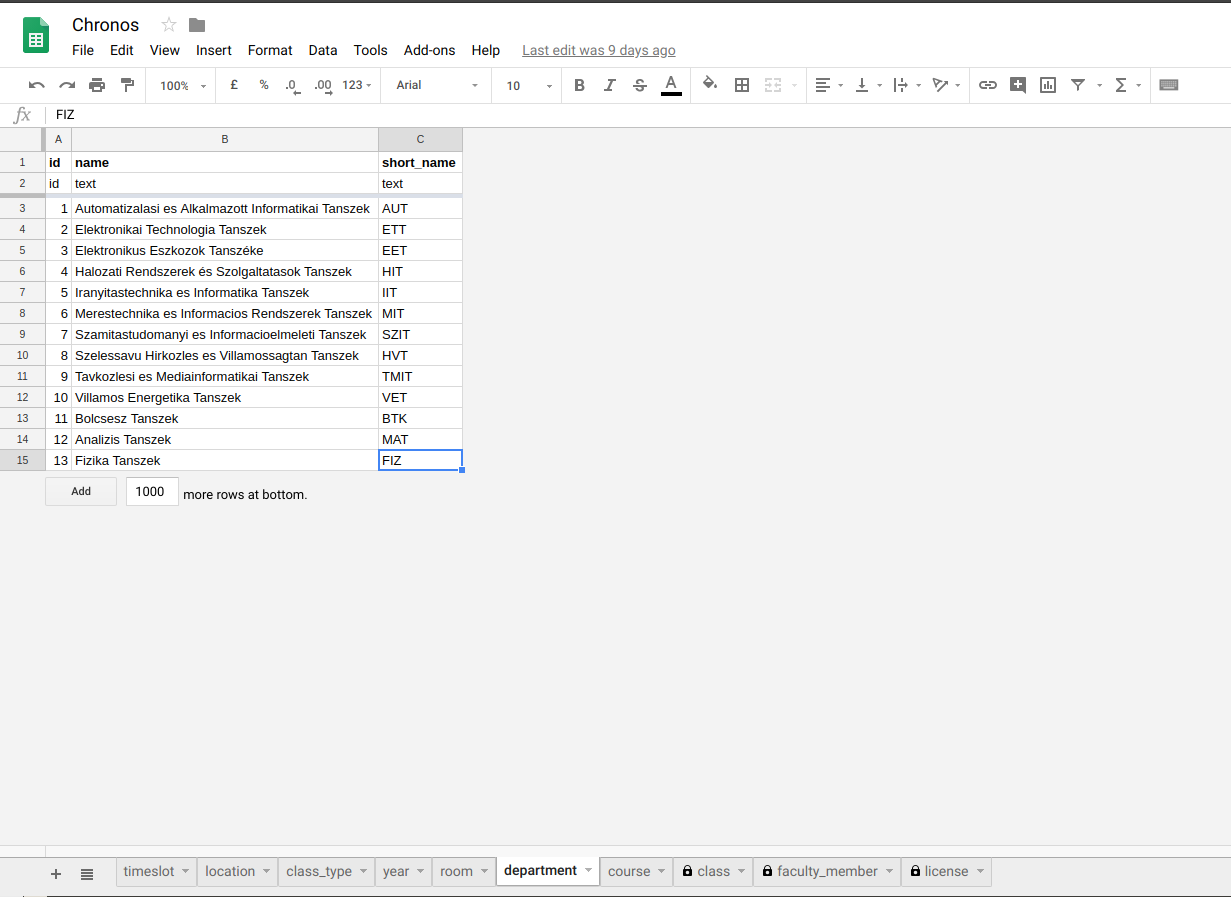
\includegraphics[width=\linewidth, keepaspectratio]{figures/chronos_sheet.png}
\caption{Google Drive Sheet} 
\label{fig:GoogleDriveSheet}
\end{figure}

The worksheets represent the classes in the data model. The first row lists the names of the variables, the second row the types of them. After that, every row is one object from the class or one row in the database. I wrote a Google Apps Script that will generate the descriptor jsons and an SQL script that creates the database structure and initialises the tables with the data from the worksheets.

Now, every time I needed to change the data model or the specific object I was able to open this spreadsheet, quickly edit it the way I wanted to, then run a few generator scripts and have my database ready and code modified to match it.

This quick prototyping method allowed me to make changes faster throughout the semester and played a huge role in completing my thesis on time.

\section{Mathematical description of the problem}

In the following section I will describe the Constraint Satisfaction Problem that I used to solve the timetabling problem.

Let $c_c$ denote the number of classes, $t_c$ the number of timeslots $r_c$ the number of rooms, $f_c$ the number of faculties and $p_c$ the number of allowed parallel non-seminar classes.\\

\subsection{Variables}

The variables are assigned in the following way.\\
\\
$T_i$ is the timeslot assigned to the ith class where $1\leq{}i\leq{}c_c$.\\
$R_i$ is the room assigned to the ith class where $1\leq{}i\leq{}c_c$.\\
$F_i$ is the faculty member assigned to the ith class where $1\leq{}i\leq{}c_c$.\\
\\
Then, there are special uniqueness variables. These variables help us to describe unique constraints in the system.  \\
\\
$U_{TR_i}$ is a uniqueness variable on the timeslot and room pair assigned to the ith class where $1\leq{}i\leq{}c_c$. These variables make sure rooms are not overbooked in any timeslot.\\\\
$U_{TF_i}$ is a uniqueness variable on the timeslot and faculty member pair assigned to the ith class where $1\leq{}i\leq{}c_c$. These variables make sure the faculty members don't have to teach two classes at the same time.\\\\
$U_{TYP_{i,j}}$ is a uniqueness variable on the timeslot, year and parallelness triplet assigned to the ith class where $1\leq{}i\leq{}c_c$ and jth parallel timeslot where $1\leq{}j\leq{}p_c$. These variables make sure that no year of students has to go to two classes at the same time.\\\\
$P_{i}$ is a parallelness variable for non-seminar classes. This allows the years of students to have parallel non-seminar classes in their timetable. \\

\subsection{Domains}

The domains of the variables are as follows.\\
\\
$T_i \in{} (1,t_c)$\\
$R_i \in{} (1,r_c) \cap \{$''where the room type matches the course type''$\}$\\
$F_i \in{} (1,f_c) \cap \{$''which class the faculty member is licensed to teach''$\}$\\
\\
$U_{TR_i} \in{} (1, (t_c + 1) (r_c + 1))$, $1\leq{}i\leq{}c_c$\\
$U_{TF_i} \in{} (1, (t_c + 1) (f_c + 1))$, $1\leq{}i\leq{}c_c$\\
$U_{TYP_{i,j}} \in{} (1, (t_c + 1) (y_c + 1) (p_c + 1))$, $1\leq{}i\leq{}c_c$, $1\leq{}j\leq{}c_c$\\

\subsection{Constraints}

The constraints are below.\\
\\
The uniqueness variables are number pairs represented as one number in a $t_c$ base-number system.\\
\\
$U_{TR_i} = R_i (t_c + 1) + T_i$\\
$U_{TF_i} = F_i (t_c + 1) + T_i$\\
\\
The $U_{TYP_i}$ variable uses the same representation trick but for a triplet.
When the ith class is a non-seminar class:\\
$U_{TYP_{i,1}} = Y_i (p_c + 1) (t_c + 1) + P_i (t_c + 1) + T_i$\\
\\
When the ith class is a seminar class we have to occupy ever parallel timeslot. This is done by creating $p_c$ number of uniqueness variables for seminars.\\
$U_{TYP_{i,j}} = Y_i (p_c + 1) (t_c + 1) + j (t_c + 1) + T_i$, $1\leq{}j\leq{}p_c$\\
\\
The following constraints make sure that the pairs and triplets are unique.\\
\\
AllDiff$(U_{TR_i})$ $\forall{}i$\\
AllDiff$(U_{TF_i})$ $\forall{}i$\\
AllDiff$(U_{TY_{i,j}})$ $\forall{}i,j$\\

\subsection{Optimalization}

To optimalize the devised timetable, I wanted to minimize the number of hole-hours for the students. To achieve this, we have to mathematically describe this using the variables in the Constraint Satisfaction Problem description above.

\paragraph{Theorem}

Let $S_1,S_2,...,S_{y_c}$ be the sets of the classes for a given year.

Minimizing $H_k = \sum\limits_{i\in{}S_k}\sum\limits_{j\in{}S_k}|T_i - T_j|$ will minimize the number of hole-hours in the kth year's timetable.

\paragraph{Lemma}

If the kth year's timetalbe with value $H_k = h$ contains a hole-hour there is always a timetable with value $H_k=h^*$ so that $h^* < h$.

\paragraph{Proof}

Let's move the chronologically first class, $min_{f}T_f$ in the timetable to the hole-hour. Then let's look at the changes in the $H_k$ value after this move. The $Y_i$, $Y_j$ pairs where $i\neq{}f$ and $j\neq{}f$ did not change, so their contribution to the sum did not change either.

The only pairs that changed are the ones where one of them was $T_f$.

Since $T_f$ was the first class, the value of $T_f$ could only increase when moved to the hole-hour.

Let $T_s$ denote the chronologically second class in the timetable. If we increase $T_f$'s value until $T_f = T_s$ the sum of every ($T_f$, $T_x$) pair's distances decreased, since $T_s\leq{}T_x$.

Then, let's denote the chornologically thrid class as $T_t$. If we increase  $T_f$'s value until $T_f = T_t$ there are two cases. The first case is with $T_s$. Since $T_f$ is getting further away from $T_s$, their distance is increasing. However, if we pair $T_s$ up with the chronologically last class, $T_l$, the sum of their distances from $T_f$ stays constant. The other case is with every other $T_x$, where the distance is decreasing.

We can continue this logic until a) we reach a hole-hour and put $T_f$ there, or b) until we leave the first half of the timetable.

In case a) we have successfully proven that the sum of all pairs's distances decreased by putting $T_f$ in the hole-hour. In case b) we know that hole-hour exists in the second half of the timetable. Here, we need to do the same process but instead of the chronologically first class we use the chronologically last and decrease its value, so from this viewpoint the hole-hour will be in the first half of the timetable.

This proves the correctness of the lemma.

Now, if for every timetable that contains a hole-hour we have proven that the $H_k$ value can't be minimal. This means that only timetables with no hole-hours can minimize the $H_k$ value, so minimizing for this results in hole-hour-less timetables.

This is the constraint I used for optimizing the timetables in the solver.

\section{Client}

The client is a simple Qt application, with minimal GUI.

\begin{figure}[!ht]
\centering
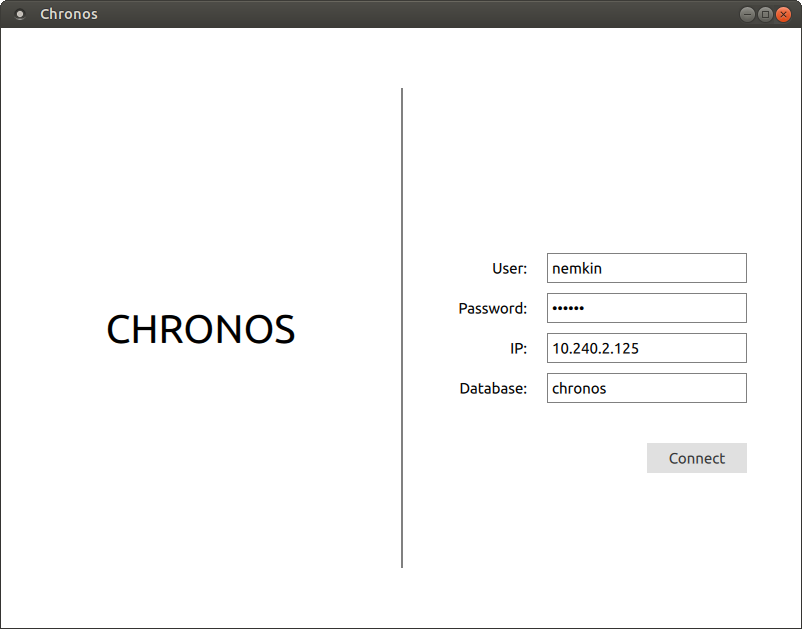
\includegraphics[width=\linewidth, keepaspectratio]{figures/login.png}
\caption{Login Screen} 
\end{figure}

\begin{figure}[!ht]
\centering
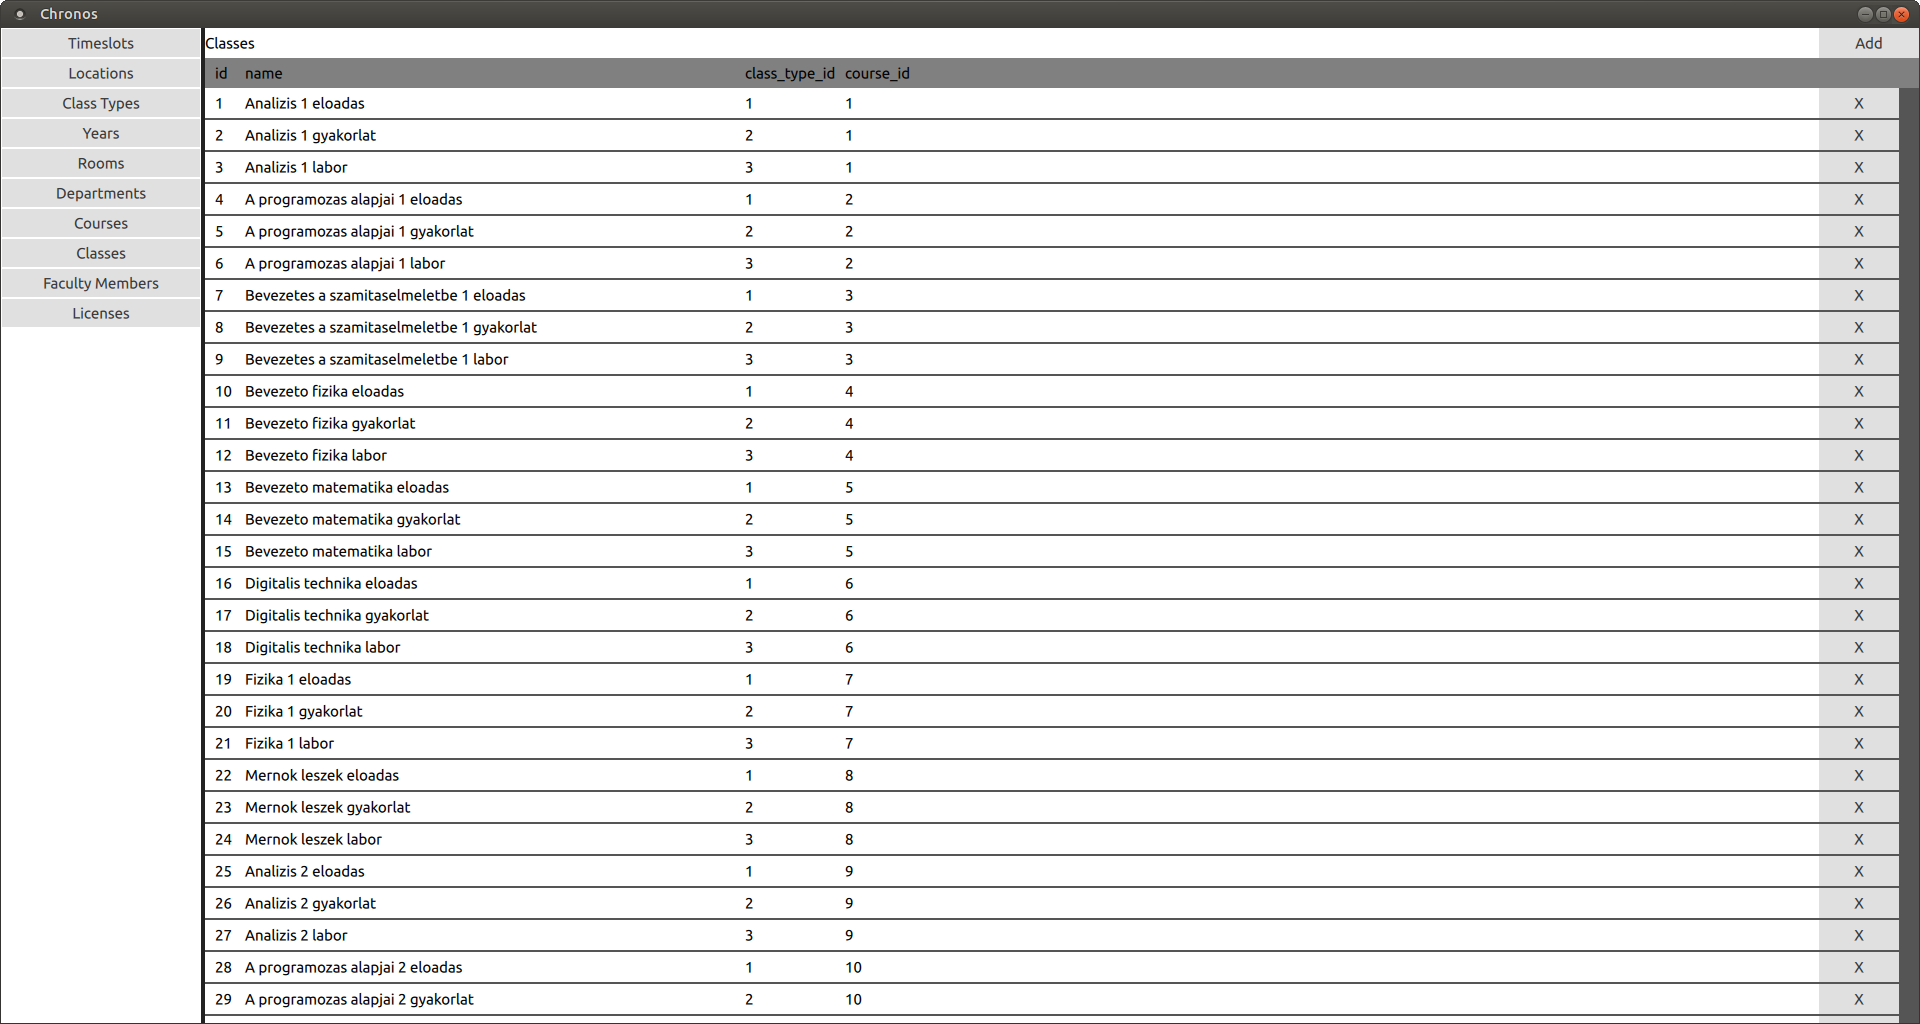
\includegraphics[width=\linewidth, keepaspectratio]{figures/inside.png}
\caption{Inside} 
\end{figure}

It can display the data, but currently it will not upload it back to the database.

\chapter{Problems and solutions}

\chapter{Results}
A megtervezett mûszaki alkotás értékelése, kritikai elemzése, továbbfejlesztési lehetõségek

introduction:

Source: https://www.vik.bme.hu/fmd/539.html
Source: https://www.bme.hu/sites/default/files/csatolmanyok/
                tenyek\_es\_adatok\_2017\_18\_mod.pdf

Thanking:
Pintér Richárd, Gyori Erzsébet, Tevesz Gábor, Asztalos Márk, Kárpinszky András, En-Co Software Kft., Nemkin Róbert.

Market analysis:

Source:
Gyori Erzsébet (requirements)
https://www.timetabler.com/
https://www.unitime.org/
https://www.youtube.com/watch?v=anUOP14l1QE
https://www.youtube.com/watch?v=0S9DQiG6hXo


Framework

Many frameworks and programming languages exist that can be used to solve problems with COP.

Declarative programming languages such as Prolog or Erlang would be a good fit. However they are hard to create UIs for and hard to connect to databases. Typical UI applications are not easy in these languages.

I choose Google's OR-tools as a toolkit because it is open source, it has a C++ framework and I wanted to use C++. Google is a company that solves these problems a lot so I thought this is they use so its good.
I choose Google's OR-tools because:
- It is open source.
- I trust Google to make good programs.
- It had many solvers not just COP so it would be convenient to change.

Architecture

The architecture consists of 3 parts:
- The database is responsible for storing every data.  I used PostgreSQL for the database since it can be run on a different computer, contains user authentication and highly convenient.

Data model:

I suspected the data model would change throughout the semester so I constructed a Python program that automatically generates my C++11 classes from a table.

Type model json:
I described  the types I can use the following way: What the C++ type should be for it, what the SQL type should be for it and the default value of it.
{
    "id": {
        "cpp": "int", 
        "sql": "SERIAL PRIMARY KEY",
        "default\_value": "0"
    },
    "reference": {
        "cpp": "int",
        "sql": "INTEGER",
        "default\_value": "0"
    },
    "int": {
        "cpp": "int",
        "sql": "INTEGER",
        "default\_value": "0"
    },
    "double": {
        "cpp": "double",
        "sql": "DOUBLE PRECISION",
        "default\_value": "0.0"
    },
    "text": {
        "cpp": "std::string",
        "sql": "TEXT",
        "default\_value": "\\"\\""
    },
    "bool": {
        "cpp": "bool",
        "sql": "BOOLEAN",
        "default\_value": "false"
    },
    "timestamp": {
        "cpp": "std::string",
        "sql": "TIMESTAMP",
        "default\_value": "\\"\\"" 
    }
}

Then my classes look like this:

Default is what every class has. Every class also has an id which is the primary key.

The references will translate to a foreign key in the database.

I changed the data model quite a lot during the semester. This way of describing it allowed me to quickly iterate through the new way of the model and so I was able to work much faster compared to having done it manually.

I also auto generated the database.

{
    "default": {
        "members": [
            {
                "name": "modified\_timestamp",
                "type": "timestamp"
            },
            {
                "name": "is\_deleted",
                "type": "bool"
            }
        ]
    },
    "classes": [
        {
            "class": "timeslot",
            "members": [
                {
                    "name": "name",
                    "type": "text"
                }
            ],
            "references": []
        },
        {
            "class": "location",
            "members": [
                {
                    "name": "name",
                    "type": "text"
                }
            ],
            "references": []
        },
        {
            "class": "class\_type",
            "members": [
                {
                    "name": "name",
                    "type": "text"
                }
            ],
            "references": []
        },
        {
            "class": "year",
            "members": [
                {
                    "name": "name",
                    "type": "text"
                }
            ],
            "references": []
        },
        {
            "class": "room",
            "members": [
                {
                    "name": "name",
                    "type": "text"
                },
                {
                    "name": "size\_type",
                    "type": "text"
                }
            ],
            "references": [
                {
                    "class": "location"
                },
                {
                    "class": "class\_type"
                }
            ]
        },
        {
            "class": "department",
            "members": [
                {
                    "name": "name",
                    "type": "text"
                },
                {
                    "name": "short\_name",
                    "type": "text"
                }
            ],
            "references": []
        },
        {
            "class": "course",
            "members": [
                {
                    "name": "name",
                    "type": "text"
                }
            ],
            "references": [
                {
                    "class": "year"
                },
                {
                    "class": "department"
                }
            ]
        },
        {
            "class": "class",
            "members": [
                {
                    "name": "name",
                    "type": "text"
                }
            ],
            "references": [
                {
                    "class": "class\_type"
                },
                {
                    "class": "course"
                }
            ]
        },
        {
            "class": "faculty\_member",
            "members": [
                {
                    "name": "name",
                    "type": "text"
                }
            ],
            "references": [
                {
                    "class": "department"
                }
            ]
        },
        {
            "class": "license",
            "members": [],
            "references": [
                {
                    "class": "course"
                },
                {
                    "class": "class\_type"
                },
                {
                    "class": "faculty\_member"
                }
            ]
        }
    ]
}

And I can create these from a simple json. Quite good.

Then I went further and created a google docs where I could just create the database and download its descriptors and the update functions.

Table screenshot.

Google script downloader.




Backend development

Simple model
https://developers.google.com/optimization/cp/original\_cp\_solver
- Original Google CP solver. Extra slow. Took 1 day. Changed it to CP solver, it took 3 minutes. Appears to be old code which is kept because in some small input cases it is better.


- Practice sessions could overlap

Mathematical equationsx
Proof of the minimalisation.

ja a bizonyítás úgy fog kinézni hogy vegyünk egy órarendet amiben van lyukas óra
erre belátjuk hogy létezik olyan óra amit a lyukasóra helyére mozgatva csökken a lyukasórák száma
válasszuk ki a legelsöt a héten és mozgassuk át a lyukas óra helyére
nyilván ilyenkor a páronkénti távolságok azokra a párokra amiben nincs benne a kiválasztott nem változtak
maradtak azok a párok amikben az egyik a kiválasztott
és akkor erre kell belátni hogy ha
kiválasztott, szám szám szám üres szám szám szám
helyett
szám szám szám kiválasztott szám szám szám van
az kisebb távolságot eredményez
erre meg tök ugyanaz a bizonyítás
mint arra hogy a számtani közép az a szám ami n db számtól vett távolság átlagát minimalizálja
erre belátjuk hogy létezik olyan óra amit a lyukasóra helyére mozgatva csökken a *páronkénti távolságok összege*
elírtam
tehát semelyik olyan órarend nem lehet minimális páronkénti távolságösszegű amiben van lyukasóra mert a lyukasóra helyére mozgatva
a legelsö órát csökkenteni lehet a páronkénti távolságokat
Q.E.D

Frontend development

Qt. Screenshots.

Tests:

Supergraphs.

Q.: Why is timetable planning a multivariable optimisation problem? Why can we use operations research to solve it?

Q.: What are multi-variable target functions? How do we optimise them?

Q.: What methods are present for multi-variable optimisation?

Q.: How can we use operations research to solve real-life problems? Why is it important?

Q.: Where do they use operations research?

Q.: What languages, frameworks are available that implement these techniques? 

Q.: Why did I choose OR-tools?


Q.: The student's job is to implement multi-variable optimisation in a timetabling application for universities.

Q.: What type of algorithm did I choose, [why did I choose that]? How I designed it?

Q.: How I implemented the algorithm?

What equalities did we use and how we implemented the server side?
- Every class has a teacher and a room assigned.
- No student or teacher has to be in more than one place at one time.
- No double-booked rooms.
- The appointed room must fit the number of students in the class and have the necessary equipment for it.

Q.: How can we verify its correctness?

Q.: How I verified it?

Q.: What example datasets I used?

Q.: How I customised the algorithm? (Did I make it faster? Better?)

Q.: How I created the user interface?

Q.: What is Qt? How can we use Qt?

Q.: What other tools I used?
- Git/Github
- VIM
- Etc?

Q: How I generate the code from the model?
Q: Bad models? Generate all proposals and throw out the ones within conflict?
Q: Non-SAT CP solver.
Q: All exercise/labours at the same timeslot.


%----------------------------------------------------------------------------
\chapter*{K�sz�netnyilv�n�t�s}\addcontentsline{toc}{chapter}{K�sz�netnyilv�n�t�s}
%----------------------------------------------------------------------------

Ez nem k�telez�, ak�r t�r�lhet� is. Ha a szerz� sz�ks�g�t �rzi, itt lehet k�sz�netet nyilv�n�tani azoknak, akik hozz�j�rultak munk�jukkal ahhoz, hogy a hallgat� a szakdolgozatban vagy diplomamunk�ban le�rt feladatokat sikeresen elv�gezze. A konzulensnek val� k�sz�netnyilv�n�t�s sem k�telez�, a konzulensnek hivatalosan is dolga, hogy a hallgat�t konzult�lja.

%\listoffigures\addcontentsline{toc}{chapter}{Ábrák jegyzéke}
%\listoftables\addcontentsline{toc}{chapter}{Táblázatok jegyzéke}

\bibliography{others/mybib}
\addcontentsline{toc}{chapter}{Bibliography}
\bibliographystyle{plain}

%----------------------------------------------------------------------------
\appendix
%----------------------------------------------------------------------------
\chapter*{F�ggel�k}\addcontentsline{toc}{chapter}{F�ggel�k}
\setcounter{chapter}{6}  % a fofejezet-szamlalo az angol ABC 6. betuje (F) lesz
\setcounter{equation}{0} % a fofejezet-szamlalo az angol ABC 6. betuje (F) lesz
\numberwithin{equation}{section}
\numberwithin{figure}{section}
\numberwithin{lstlisting}{section}
%\numberwithin{tabular}{section}

%----------------------------------------------------------------------------
\section{A TeXnicCenter fel�lete}
%----------------------------------------------------------------------------
\begin{figure}[!ht]
\centering
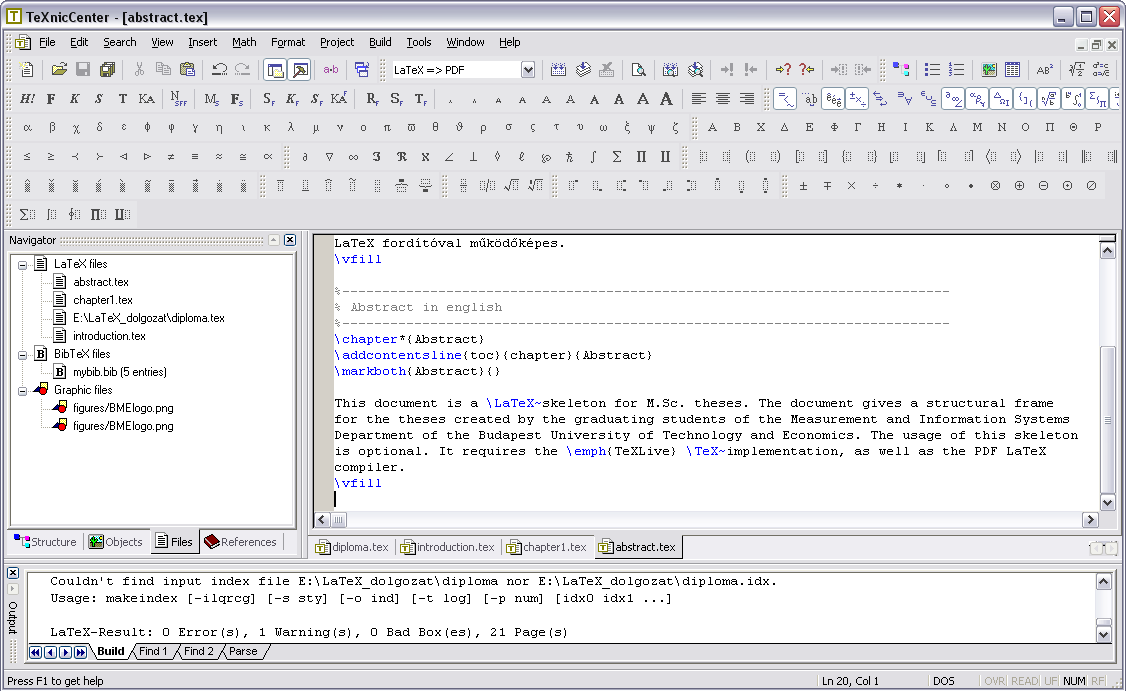
\includegraphics[width=150mm, keepaspectratio]{figures/TeXnicCenter.png}
\caption{A TeXnicCenter Windows alap� \LaTeX-szerkeszt�.} 
\end{figure}

%----------------------------------------------------------------------------
\clearpage\section{V�lasz az ,,�let, a vil�gmindens�g, meg minden'' k�rd�s�re}
%----------------------------------------------------------------------------
A Pitagorasz-t�telb�l levezetve
\begin{align}
c^2=a^2+b^2=42.
\end{align}
A Faraday-indukci�s t�rv�nyb�l levezetve
\begin{align}
\rot E=-\frac{dB}{dt}\hspace{1cm}\longrightarrow \hspace{1cm}
U_i=\oint\limits_\mathbf{L}{\mathbf{E}\mathbf{dl}}=-\frac{d}{dt}\int\limits_A{\mathbf{B}\mathbf{da}}=42.
\end{align}







\label{page:last}
\end{document}

